\usetikzlibrary{chains,positioning,fit,arrows}
\begin{document}
\title{Übungsblatt~6}
\subtitle{Schlüssel -- R-Baum, Function Based Index}
\maketitle
\section*{Lernziele}
\begin{itemize}
	\item Auftretende Probleme bei nicht isolierten Transaktionen
	\item Möglichkeiten, diese Probleme zu erkennen und zu vermeiden
	\item Möglichkeiten zur Recovery unter Verwendung von Logs
\end{itemize}


\section*{Literatur}
\HaerderNintyNine{14}

\ElmasriFive{18, insbes. 18.1}

\GarciaMolinaFirst{18}

\BerensonNintyFive

\section{Fragen zur Vorlesung}

\begin{enumerate}[a)]
	\item Welche möglichen Probleme bei der gleichzeitigen Ausführung von Transaktionen haben Sie in der Vorlesung kennengelernt?

\begin{solution}
\begin{itemize}
	\item Verlorengegangene Änderung (Dirty Write, Lost Update)
	\item Lesen nicht freigegebener Änderungen (Dirty Read)
	\item Inkonsistente Analyse (Non-Repeatable Read)
	\item Phantom-Problem
\end{itemize}
Für die Anomalien im Mehrbenutzerbetrieb gibt man bestimmte Abläufe,
d.\,h.\ Ausführungsreihenfolgen von Operationen verschiedener Transaktionen,
als Muster an.
Beinhaltet ein Ablauf das Muster einer Anomalie,
so sagt man:
Die Anomalie tritt in diesem Ablauf auf.

Leider ist die Definition der Anomalie-Muster umstritten.
Das zeigt sich u.\,a.\ daran, dass viele reale Systeme (z.\,B.\ Oracle, PostgreSQL) nach unserer Definition nicht serialisierbar (und damit möglicherweise nicht korrekt) arbeiten, da sie eine andere Definition verwenden.
Für eine tiefere Beschäftigung mit dieser Tatsache sei der Artikel von Berenson et al.\ empfohlen.
Für diese Veranstaltung ist das aber nicht notwendig.

Da aber eine Definition von Anomalie-Abläufen nötig ist, um über Anomalien sprechen zu können, verwenden wir die Definitionen aus dem Artikel von Berenson et al. (Vorlesungsfolie~\AnomalieDef):

\paragraph{\color{solutioncolor}Dirty Write}
$w_1[x] \ldots w_2[x] \ldots
((c_1 \textrm{ oder } a_1) \textrm{ und } (c_2 \textrm{ oder } a_2)$
in beliebiger Reihenfolge)

Zwei Transaktionen schreiben überschneidend dasselbe Datenelement,
wodurch Inkonsistenzen entstehen können
und das Rücksetzen von Transaktionen erschwert wird.

\paragraph{\color{solutioncolor}Dirty Read}
$w_1[x] \ldots r_2[x] \ldots
((c_1 \textrm{ oder } a_1) \textrm{ und } (c_2 \textrm{ oder } a_2)$
in beliebiger Reihenfolge)

Transaktion~2 hat Daten gelesen, die inkonsistent zu anderen Daten sein können und die eventuell "`nie existiert haben"', da Transaktion~1 abgebrochen werden könnte und damit alle ihre Änderungen rückgängig gemacht werden.

\paragraph{\color{solutioncolor}Non-Repeatable Read}
$r_1[x] \ldots w_2[x] \ldots
((c_1 \textrm{ oder } a_1) \textrm{ und } (c_2 \textrm{ oder } a_2)$
in beliebiger Reihenfolge)

Transaktion~1 sieht, wenn sie erneut liest, einen anderen Wert als zuvor. Dadurch kann es zu inkonsistenten Analysen kommen.

\paragraph{\color{solutioncolor}Phantom-Problem}
$r_1[P] \ldots w_2[y \textrm{ in } P] \ldots
((c_1 \textrm{ oder } a_1) \textrm{ und } (c_2 \textrm{ oder } a_2)$
in beliebiger Reihenfolge);
$P$ steht hier für die Menge der Datenobjekte, die ein Prädikat erfüllen.

Nachdem Transaktion~1 $P$ liest, verändert Transaktion~2 diese Menge durch Einfügen eines geeigneten Tupels, wodurch inkonsistente Analysen entstehen können.
\end{solution}

\begin{note}
Eine Anomalie liegt unabhängig davon vor, ob die Transaktionen mit Abort oder Commit enden, und unabhängig von der Reihenfolge des Endes. Damit die Anomalie vorliegt, dürfen beide Transaktionen aber erst \emph{nach} den anderen Operationen (z.\,B.\ $(r_1[x] w_2[x])$ bei Non-Repeatable Read) enden. Der Ablauf $(r_1[x] c_1[x] w_2[x] a_2[x])$ ist also kein Non-Repeatable Read, der Ablauf $(r_1[x] w_2[x] c_1[x] a_2[x])$ schon.

Das Datenbanksystem kann nicht prüfen, ob eine Anomalie zu einem Problem wird oder nicht, da es nicht weiß, was das Anwendungsprogramm mit den Daten macht. Sobald eine Anomalie vorliegt, besteht aber die Möglichkeit, dass ein Problem, also ein anderes Ergebnis als bei einem seriellen Ablauf, entsteht. Deshalb muss das Datenbanksystem Abläufe mit Anomalien verhindern. Umgekehrt betrachtet muss also in jedem Ablauf, der zu einem Problem führt, eine Anomalie vorliegen.

Beispiel für ein Non-Repeatable Read (und dafür, warum nach Berenson et al.\ kein zweites $(r_1[x])$ gefordert wird), direkt aus Berenson et al.:

x und y seien zwei Kontostände, T1 möchte die Summe der beiden Kontostände ermitteln, T2 nimmt eine Umbuchung von 40 von x auf y vor.

$(r_1[x=50] r_2[x=50] w_2[x=10] r_2[y=50] w_2[y=90] c_2 r_1[y=90] c_1)$

T1 sieht eine Summe von 140 statt der korrekten 100. Die Anomalie ist ein Non-Repeatable Read aufgrund von $(r_1[x=50] \ldots w_2[x=10] \ldots c_2 \ldots c_1)$
Würde Non-Repeatable Read ein zweites $(r_1[x])$ erfordern, würde in dem Ablauf keine Anomalie auftreten.

Zentraler Punkt in Berenson et al., \emph{A Critique of ANSI SQL Isolation Levels} ist folgender:
Einige Anomalien werden durch den SQL-Standard wie folgt definiert:
\begin{enumerate}[i)]
  \item P1 ("`Dirty read"'): SQL-transaction $T_1$ modifies a row. SQL-transaction $T_2$ then reads that row before $T_1$ performs a COMMIT. If $T_1$ then performs a ROLLBACK, $T_2$ will have read a row that was never committed and that may thus be considered to have never existed.

  \item P2 ("`Non-repeatable read"'): SQL-transaction $T_1$ reads a row. SQL-transaction $T_2$ then modifies or deletes that row and performs a COMMIT. If $T_1$ then attempts to reread the row, it may receive the modified value or discover that the row has been deleted.

  \item P3 ("`Phantom"'): SQL-transaction $T_1$ reads the set of rows N that satisfy some $<$search condition$>$. SQL-transaction $T_2$ then executes SQL-statements that generate one or more rows that satisfy the $<$search condition$>$ used by SQL-transaction $T_1$. If SQL-transaction $T_1$ then repeats the initial read with the same $<$search condition$>$, it obtains a different collection of rows.
\end{enumerate}

Dabei ist nun ungeklärt, ob der jeweilige "`If"'-Teil zur Definition der Anomalie gehört oder nur eine Erklärung dessen darstellt, was bei Auftreten der Anomalie passieren kann. Konkret: Muss $T_1$ ein ROLLBACK durchführen, damit ein Dirty Read vorliegt? Oder liegt der bereits durch $w_1(x) r_1(x)$ vor und der "`If $T_1$ \ldots "'-Satz erläutert nur, warum das schlimm sein kann? Genau das ist umstritten. Aber für uns gelten die Definitionen, die oben angegeben sind.
\end{note}

\item Definieren Sie den Begriff "`Serialisierbarkeit"'.

\begin{solution}
Direkt aus den Vorlesungsfolien:
Ein Schedule von Transaktionen ist serialisierbar, wenn er zu irgendeinem seriellen Ablauf der in ihm enthaltenen Transaktionen äquivalent ist.
\end{solution}


\item Seien $T_i$ und $T_j$ beliebige Transaktionen und $H$ und $G$ zwei
  dazugehörige Abläufe. Markieren Sie die Bedingungen, die für alle
  Operationen auf einem beliebigen Datenobjekt $A$ gelten müssen, damit
  zwei Abläufe nach der Definition der Vorlesung "`äquivalent"' sind.
  \nt{Studierende darauf Hinweisen, dass in der Klausur ausgefüllt und nicht gekreuzt wird. Korrekturen mit Korrekturband.}

  \begin{itemize}
    \itemmc   \hspace*{0.45em} $r_i[A] <_H r_j[A] \Leftrightarrow r_i[A] <_G r_j[A]$
    \itemmcsol \hspace*{0.45em} $r_i[A] <_H w_j[A] \Leftrightarrow r_i[A] <_G w_j[A]$
    \itemmcsol \hspace*{0.45em} $w_i[A] <_H r_j[A] \Leftrightarrow w_i[A] <_G r_j[A]$
    \itemmcsol \hspace*{0.45em} $w_i[A] <_H w_j[A] \Leftrightarrow w_i[A] <_G w_j[A]$
  \end{itemize}

\item Geben Sie eine Möglichkeit an, Serialisierbarkeit zu gewährleisten.

\begin{solution}
Serialisierung oder Sperren.
Abhängigkeitsgraphen zählen nicht, da sie zur Prüfung dienen.
Sicherstellen muss man das dann noch auf anderem Wege.
\end{solution}

\begin{note}
Aus didaktischen Gründen lassen wir den Unterschied zwischen Konflikt-Serialisierbarkeit und anderen Serialisierbarkeitsarten aus.
Ersteres ist ein stärkeres Kriterium und wird sowohl durch Abhängigkeitsgraphen als auch durch 2PL gewährleistet.
Wir verbieten also einige Abläufe, die wir eigentlich erlauben könnten.
Grund: Konflikt-Serialisierbarkeit ist leichter zu prüfen.
\end{note}

\end{enumerate}


\section{Höhe von B-Bäumen}
Geben Sie für den B-Baum eine Formel an, mit der man die obere und untere Schranke für die Höhe des Baums aus gegebenem $k$ und der Anzahl der eingetragenen Sätze oder Satzadressen $n$ bestimmen kann ($n\in\mathbb{N}_1$).

\begin{solution}

\subsection*{Obere Schranke für die Höhe des B-Baums}
\begin{tabular}{p{2cm} p{8cm}}
	Tiefe			& Minimale Knotenzahl in der Tiefe		\\
	\hline
	1				& 1 														\\
	\hline
	2 				& $2(k+1)^0$ 										\\
	\hline
	3 				& $2(k+1)^1$  									\\
	\hline
	4 				& $2(k+1)^2$ 										\\
	\hline
	\ldots 		& \ldots												\\
	\hline
	h 				& $2(k+1)^{h-2}$ 								\\
	\hline
\end{tabular}

Definition geometrische Reihe:
\begin{align*}
\sum_{i=0}^n q^i &= \frac{q^{n+1}-1}{q-1}
\end{align*}
Minimale Knotenzahl im Baum bei gegebener Höhe =
Summe über Minimalzahl der einzelnen Ebenen

\begin{align*}
1 + \sum_{i = 2}^h 2\cdot (k + 1)^{i-2} = 1 + \sum_{i  = 0}^{h-2} 2 \cdot (k +1)^{i}
\overset{\text{geometr.}}{\underset{\text{Reihe}}{=}} 1 + 2 \cdot \frac{(k +1)^{h-1} - 1}{k + 1 - 1}
= 1 + 2 \cdot \frac{(k + 1)^{h - 1} - 1}{k}
\end{align*}

Minimale Anzahl der Elemente (TIDs) im Baum =
$\mathrm{Knotenzahl} \cdot k$ (jeder Knoten minimal gefüllt)
\begin{align*}
1 + k \cdot 2 \frac{(k + 1)^{h - 1} - 1}{k} = 1 + 2 \cdot (k + 1)^{h - 1} - 2 = 2 \cdot (k + 1)^{h - 1} - 1
\end{align*}
Wurzel kann auch weniger als $k$ Elemente beinhalten.

Es gilt also:
\begin{align*}
2 \cdot (k + 1)^{h - 1} - 1 &\leq n\\
2 \cdot (k + 1)^{h - 1} &\leq n + 1\\
(k + 1)^{h - 1} &\leq \frac{n + 1}{2}\\
h - 1 &\leq \log_{k +1} \text{\huge{(}}\frac{n + 1}{2}\text{\huge{)}}\\
h &\leq \log_{k +1} \text{\huge{(}}\frac{n + 1}{2}\text{\huge{)}} + 1
\end{align*}

Damit erhalten wir:
\begin{align*}
h_{oben}(n):= & \log_{k +1} \text{\huge{(}}\frac{n + 1}{2}\text{\huge{)}} + 1
\end{align*}


\subsection*{Untere Schranke für die Höhe des B-Baums}
\begin{tabular}{p{2cm} p{8cm}}
	Tiefe			& Maximale Knotenzahl in der Tiefe	\\
	\hline
	1				& 1 = $(2k + 1)^0$ 							\\
	\hline
	2 				& $(2k+1)^1$ 										\\
	\hline
	3 				& $(2k+1)^2$ 										\\
	\hline
	4 				& $(2k+1)^3$ 										\\
	\hline
	\ldots		& \ldots												\\
	\hline
	h 				& $(2k+1)^{h-1}$ 								\\
	\hline
\end{tabular}

Maximale Knotenzahl im Baum =
Summe über Maxima je Ebene
\begin{align*}
\sum_{i = 1}^{h} (2k + 1)^{i - 1} = \sum_{i = 0}^{h - 1} (2k + 1)^{i} \overset{\text{geometr.}}{\underset{\text{Reihe}}{=}} \frac{(2k + 1)^h - 1}{2k + 1 - 1} = \frac{(2k + 1)^h - 1}{2k}
\end{align*}
Maximale Anzahl der Elemente(TIDs) im Baum =
$\mathrm{Knotenzahl} \cdot 2k$ (jeder Knoten voll gefüllt)

\begin{align*}
2k \cdot \frac{(2k + 1)^h - 1}{2k} = (2k + 1)^h - 1
\end{align*}
Es gilt also:
\begin{align*}
(2k + 1)^h - 1 &\geq n\\
(2k + 1)^h &\geq n + 1\\
h & \geq \log_{2k + 1} (n +1)
\end{align*}
Damit erhalten wir:
\begin{align*}
h_{unten}(n):=& \log_{2k + 1} (n +1)
\end{align*}
% Ein Comment darf andscheinend eine maximale länge nicht überschreiten, daher zwei...
\end{solution}
\begin{solution}
\subsection*{Was bedeutet das nun?}
Beispiel:
\begin{itemize}
	\item Blockgröße: 4\,kiB
	\item Schlüssellänge: 10\,B
	\item Blockzeiger: 4\,B (erlaubt bei dieser Blockgröße Files bis ca. 16\,TiB)
	\item TID: 5\,B (Blockzeiger + 1\,B für die Satznummer)
	\item Satz: 117\,B
\end{itemize}
Daraus ergeben sich für k:

\begin{tabular}{p{4cm} p{2cm} p{3.5cm} p{3.5cm}}
										& B-Baum 	& B*-Baum Knoten	& B*-Baum Blatt	\\
	\hline
	Primärorganisation 		& 15 			& 146 						& 16 					\\
	\hline
	Sekundärorganisation 	& 107 			& 146 						& 136					\\
	\hline
\end{tabular}

Rechenweg:
\begin{align*}
\text{Größe B-Baum Knoten} &= 
((2k + 1) \cdot \text{Blockzeiger} + 2k \cdot \text{Schlüssel} + 2k \cdot \text{(TID oder Satz)})\\
&= 2k \cdot (\text{Blockzeiger} + \text{Schlüssel} + \text{(TID oder Satz)}) + \text{Blockzeiger}\\
&= 2k \cdot (4 + 10 + (5\text{ oder }117)) + 4 \text{[Byte]} = 2k \cdot (19\text{ oder }131) + 4 \text{[Byte]}\\
\text{TID}_{k = 107} &=2 \cdot 107 \cdot 19 + 4 = 4070\\
\text{TID}_{k = 108} &=2 \cdot 108 \cdot 19 + 4 = 4108\\
\text{Satz}_{k = 15} &= 2 \cdot 15 \cdot 131 + 4 = 3934\\
\text{Satz}_{k = 16} &= 2 \cdot 16 \cdot 131 + 4 = 4196\\
\text{B*-Knoten}_{k=146} &= 2\cdot 146 \cdot (4 + 10) + 4 = 4092\\
\text{B*-Blatt-TID}_{k=136} &= 2\cdot 136\cdot (10+5) = 4080\\
\text{B*-Blatt-Satz}_{k=16} &= 2\cdot 16\cdot (10+117) = 4064\\
\text{B*-Blatt-Satz}_{k=17} &= 2\cdot 17\cdot (10+117) = 4318\\
\end{align*}

\begin{note}
Die Werte alle zu bestimmen dauert 10-15 Minuten! Danach können wir kein Beispiel rechnen. $\rightarrow$ Werte angeben und dann die Höhe bestimmen.
\end{note}

Für 1.000.000 Datensätze ergibt sich:

\begin{tabular}{p{4cm} p{3cm} p{3cm}}
	B-Baum-Höhe				& min 						& max						\\
	\hline
	Primärorganisation 		& $4,023169201$	& $5,732892503$ 	\\
	\hline
	Sekundärorganisation 	& $2,572415323$	& $3,802647713$	\\
	\hline
\end{tabular}

Erkenntnis: Als Sekundärorganisation hat der B-Baum häufig eine Tiefe von 3, bei 100.000.000 immer noch nur 4.
Der B*-Baum ist noch etwas flacher (insbesondere als Primärorganisation), aber das betrachten wir nicht in dieser Übung.
\end{solution}


\begin{deeper}
\section{Höhe von B*-Bäumen}
Geben Sie für den B*-Baum eine Formel an, mit der man die obere und untere Schranke für die Höhe des Baums aus gegebenem k, $k_{Leaf}$ und der Anzahl der eingetragenen Sätze oder Satzadressen n bestimmen kann.

\begin{note}
\subsection*{Obere Schranke für B*-Bäume}
\begin{tabular}{cc}
	Tiefe & Minimale Blattknotenzahl in der Tiefe \\
	\hline
	1 & 1 \\
	\hline
	2 & $2\cdot (k+1)^0$ \\
	\hline
	3 & $2\cdot (k+1)^1$ \\
	\hline
	4 & $2\cdot(k+1)^2$ \\
	\hline
	\vdots & \vdots \\
	\hline
	h & $2(k+1)^{h-2}$ \\
	\hline
\end{tabular}

Minimale Anzahl der Elemente im Baum = $Blattknotenzahl \cdot k_{Leaf}$ (Jeder Knoten minimal gefüllt); Ausnahme: Höhe 1.

Damit gilt für die Obere Schranke:\\
Anmerkung Sonderbehandlung bei Höhe 1;
n ist zu klein für die Ebene darüber, also:
\begin{align*}
n&< \textrm{min\_Einträge}(h+1)\\
n&< 2\cdot(k+1)^{h-1}\cdot k_{Leaf} && 2\cdot k_{Leaf}>0\\
\frac{n}{2\cdot k_{Leaf}} &< (k+1)^{h-1} && \textrm{Log ist streng monoton steigend}\\
\log_{k+1} (\frac{n}{2\cdot k_{Leaf}}) &< h-1\\
\log_{k+1} (\frac{n}{2\cdot k_{Leaf}}) +1 &<h; && \textrm{für $x\in{\mathbb{R}}$ gilt:} \\
\textrm{da } h>1 \textrm{ und }h&\textrm{ maximal gewählt wurde}  && \min_{z\in\mathbb{Z}} (z) > x\Leftrightarrow x+1 \geq\max_{z\in\mathbb{Z}}(z);\\
h&\leq \log_{k+1}(\frac{n}{2\cdot k_{Leaf}}) +2
\end{align*}
Gültig nur für $h\in\mathbb{N}_2$, also
\begin{align*}
2&\leq 2+\log_{k+1}(\frac{n}{2\cdot k_{Leaf}})\\
0&\leq \log_{k+1} (\frac{n}{2\cdot k_{Leaf}}) && \textrm{Exp ist streng monoton steigend}\\
1&\leq \frac{n}{2\cdot k_{Leaf}} && 2\cdot k_{Leaf}>0\\
2\cdot k_{Leaf}&\leq n
\end{align*}
Somit benötigen wir für $n<2\cdot k_{Leaf}$ eine extra Funktion:\\
$h_{oben}(n):=1$ da wir hier immer nur einen Blattknoten haben.\\
Insgesamt ergibt dies:\\
\begin{align*}
h_{oben}(n): =  &1& &\textrm{wenn }n<2\cdot k_{Leaf}\\
 &\log_{k+1}(\frac{n}{2\cdot k_{Leaf}})+2& & sonst
\end{align*}
\subsection*{Untere Schranke}
\begin{tabular}{cc}
	Tiefe & Maximale Blattknotenzahl in der Tiefe \\
	\hline
	1 & 1 \\
	\hline
	2 & $(2k+1)$ \\
	\hline
	3 & $(2k+1)^2$ \\
	\hline
	4 & $(2k+1)^3$ \\
	\hline
	\vdots & \vdots \\
	\hline
	h & $(2k+1)^{h-1}$ \\
	\hline
\end{tabular}

Maximale Anzahl der Elemente im Baum = $Blattknotenzahl \cdot 2\cdot k_{Leaf}$ (Jeder Knoten maximal gefüllt);

Damit gilt für die Untere Schranke:\\
Anmerkung: Sonderbehandlung bei Höhe 1;\\
n ist zu groß für die Ebene darunter, also:
\begin{align*}
n&> \textrm{max\_Einträge}(h-1)&& \textrm{Fordert wieder Sonderbehandlung von Höhe h=1}\\
n&> (2k+1)^{h-2}\cdot 2\cdot k_{leaf}&& 2*k_{leaf} >0\\
\frac{n}{2\cdot  k_{Leaf}} &> (2k+1)^{h-2} && \textrm{Log ist streng monoton steigend}\\
\log_{2k+1} (\frac{2}{2\cdot k_{Leaf}}) &> h-2\\
\log_{2k+1} (\frac{2}{2\cdot k_{Leaf}}) +2 &>h; && \textrm{für $x\in{\mathbb{R}}$ gilt:} \\
\textrm{da } h>1 \textrm{ und }h&\textrm{ minimal gewählt wurde}  && \min_{z\in\mathbb{Z}} (z) \geq x\Leftrightarrow x+1 >\max_{z\in\mathbb{Z}}(z);\\
h&\geq 1+\log_{2k+1}(\frac{n}{2\cdot k_{Leaf}})
\end{align*}
Gültig wieder nur für $h\in\mathbb{N}_2$

Für $n<2\cdot k_{Leaf}$ ist die Schranke wieder durch $h_{unten}(n):=1$ gegeben.\\
Insgesamt ergibt dies:\\
\begin{align*}
h_{unten}(n): = & 1 &&\textrm{wenn }n<2\cdot k_{Leaf}\\
& 1+\log_{2k+1}(\frac{n}{2\cdot k_{Leaf}}) && sonst
\end{align*}
\end{note}

\end{deeper}

\beamertxt{\pagebreak}
\section{R-Bäume}
R-Bäume funktionieren ähnlich wie B*-Bäume, erlauben jedoch mehrdimensionale Indizes.
Diese können z.B. für die Indexierung von Flächen auf einer Landkarte genutzt werden (Kataster).
Die maximale Kapazität eines Knotens (sowohl Blatt als auch innerer) wird dabei mit $M$ bezeichnet.
Die minimale Auslastung eines Knotens beträgt $m$, das wir für diese Übung als $m = \lfloor\frac{M}{2}\rfloor$ wählen.

\paragraph{Hinweis:} Der R-Baum wird in der Vorlesung nicht behandelt.
Gerne können Sie die Primärliteratur verwenden\footnote{\url{https://doi.org/10.1145/602259.602266}}.

\begin{solution}
	Zunächst ein paar allgemeine Anmerkungen zu Vorgehen und Algorithmen.

	Der B*-Baum ist der eindimensionale Spezialfall eines R-Baums.

	Der wichtigste Algorithmus ist das Auffinden von Einträgen.
	Dazu geht man folgendermaßen vor:
	\begin{enumerate}
		\item Als Eingabe für den Suchalgorithmus dient ein Rechteck R.
		Gesucht werden alle Einträge, die R schneiden.
		(Alternativ könnte auch spezifiziert werden, dass nur Einträge gesucht werden, die komplett in R liegen o.\,ä.)
		\item Sei L die Wurzel.
		\item Falls L ein Blatt ist, gebe alle Einträge aus L zurück, die R schneiden.
		\item Ansonsten durchsuche alle Teilbäume, deren Eintrag in L das Suchrechteck R schneidet, mit diesem Algorithmus.
	\end{enumerate}

	Um dem Baum einen neuen Eintrag hinzuzufügen, muss zunächst das minimale Rechteck bestimmt werden, das den Eintrag komplett enthält.
	Im Baum werden nur Rechtecke und Zeiger (in inneren Knoten auf einen Teilbaum oder in Blattknoten auf ein Datenelement) gespeichert.

	Der Einfügealgorithmus für einen Eintrag mit minimalem umgebenden Rechteck R sieht grob beschrieben so aus:
	\begin{enumerate}
		\item Sei L die Wurzel.
		\item 
		\begin{enumerate}
			\item \label{insert:L}Wenn L ein Blatt ist, füge den Eintrag in L ein. \\
			Ansonsten suche den Eintrag E in L, dessen Rechteck so wenig wie möglich vergrößert werden muss, um R einzufügen.
			\item Setze L gleich dem Kindknoten, auf den der eben gewählte Eintrag zeigt, und gehe zu Schritt \ref{insert:L}.
		\end{enumerate}
		\item Ist nun im gewählten Blatt ein Überlauf entstanden, muss dieses gesplittet werden.
	\end{enumerate}

	Der Splitt verläuft analog zum Splitt in B*-Bäumen.

	Bei einem Splitt werden die Einträge des gewählten Blattknotens L so auf
	zwei neue Knoten aufgeteilt, dass es bei einem zukünftigen Zugriff möglichst
	unwahrscheinlich ist, dass beide Knoten durchsucht werden müssen.

	Entsteht bei einem Splitt ein Überlauf in einem inneren Knoten, so wird dieser genauso behandelt wie im Blattknoten.
\end{solution}


%% Vorlagen für die Zeichnungen
% circle radius
\newdimen\R
\R=0.5cm

\newcommand{\nodeA} {
	\draw (1.5, 4.5) circle (\R) node {A};
}
\newcommand{\nodeB} {
	\draw[xshift=5cm,yshift=4.3cm] (0:\R) \foreach \x in {72,144,...,359} {
		-- (\x:\R)
	} -- cycle (0:\R) node {B \hspace{0.8cm} } ;
}
\newcommand{\nodeC} {
	\draw (2  , 3.3) circle (\R) node {C};
}
\newcommand{\nodeD} {
	\draw (5  , 2.5) circle (\R) node {D};
}
\newcommand{\nodeE} {
	\draw[xshift=1.6cm,yshift=1.7cm] (0:\R) \foreach \x in {120,240} {
		-- (\x:\R)
	} -- cycle (0:\R) node {E \hspace{0.9cm} } ;
}
\newcommand{\nodeF} {
	\draw (0.9, 3.2) circle (\R) node {F};
}
\newcommand{\nodeG} {
	\draw (2.7, 1.0) circle (\R) node {G};
}
\newcommand{\nodeEred} {
	\draw[color=red,xshift=1.6cm,yshift=1.7cm] (0:\R) \foreach \x in {120,240} {
		-- (\x:\R)
	} -- cycle (0:\R) node {E \hspace{0.9cm} } ;
}
\newcommand{\nodeFred} {
	\draw[color=red] (0.9, 3.2) circle (\R) node {F};
}
\newcommand{\nodeGred} {
	\draw[color=red] (2.7, 1.0) circle (\R) node {G};
}


\newcommand{\RA} {
	\draw (1  , 4  ) rectangle (2  , 5  ) node[pos=0.9,anchor=south east] {R1};
}
\newcommand{\RB} {
	\draw (4.56, 3.8) rectangle (5.5, 4.8) node[pos=0.9,anchor=south east] {R2};
}
\newcommand{\RC} {
	\draw (1.5, 3.8) rectangle (2.5, 2.8) node[pos=0.9,anchor=north east] {R3};
}
\newcommand{\RD} {
	\draw (4.5, 3.0) rectangle (5.5, 2.0) node[pos=0.9,anchor=north east] {R4};
}
\newcommand{\RE} {
	\draw (1.32, 2.2) rectangle (2.1, 1.2) node[pos=0.9,anchor=north east] {R5};
}
\newcommand{\RF} {
	\draw (0.4, 3.7) rectangle (1.4, 2.7) node[pos=0.9,anchor=north east] {R8};
}
\newcommand{\RG} {
	\draw (2.2, 1.5) rectangle (3.2, 0.5) node[pos=0.9,anchor=north east] {R9};
}


Gegeben sei ein anfangs leerer R-Baum mit $M=4$ sowie die geometrischen Objekte A bis G im zweidimensionalen Raum:

\begin{center}
	\begin{tikzpicture}
		% border
		\draw (0,0) rectangle (6,6);

		\nodeA
		\nodeB
		\nodeC
		\nodeD
		\nodeEred
		\nodeFred
		\nodeGred

	\end{tikzpicture}
\end{center}

\begin{enumerate}[a)]
	\item Fügen Sie die Einträge A bis D ein.

	\begin{solution}
		Bisher ist nur der Wurzelknoten gefüllt:
		\begin{center}
			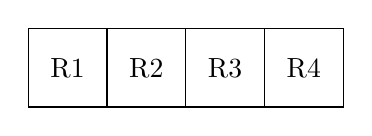
\begin{tikzpicture}
				\draw (0,0) rectangle (1,1) node[pos=.5] {R1};
				\draw (1,0) rectangle (2,1) node[pos=.5] {R2};
				\draw (2,0) rectangle (3,1) node[pos=.5] {R3};
				\draw (3,0) rectangle (4,1) node[pos=.5] {R4};
			\end{tikzpicture}
		\end{center}

		Die minimalen Rechtecke:
		\begin{center}
			\begin{tikzpicture}
				% border
				\draw (0,0) rectangle (6,6);

				\nodeA
				\nodeB
				\nodeC
				\nodeD

				\RA
				\RB
				\RC
				\RD
			\end{tikzpicture}
		\end{center}
	\end{solution}

	\item
	Fügen Sie anschließend die Einträge E, F und G in dieser Reihenfolge ein.


	\begin{solution}
		\paragraph{Einfügen von E}
		Das Einfügen von E führt zu einem Überlauf im Wurzelknoten, der gesplittet werden muss.
		Dazu müssen zwei neue Rechtecke über die bisherigen gelegt werden, die jeweils eine Teilmenge der vorhandenen Rechtecke überdecken.

		\begin{center}
			\begin{tikzpicture}
				% border
				\draw (0,0) rectangle (6,6);

				\nodeA
				\nodeB
				\nodeC
				\nodeD
				\nodeE

				\RA
				\RB
				\RC
				\RD

				\RE

				% root node
				\draw[color=green] (1  , 1.2) rectangle (2.5, 5  ) node[anchor=south] {R6};
				\draw[color=green] (4.5, 2.0) rectangle (5.5, 4.8) node[anchor=south] {R7};

			\end{tikzpicture}
		\end{center}

		Der Baum sieht dann so aus:
		\begin{center}
			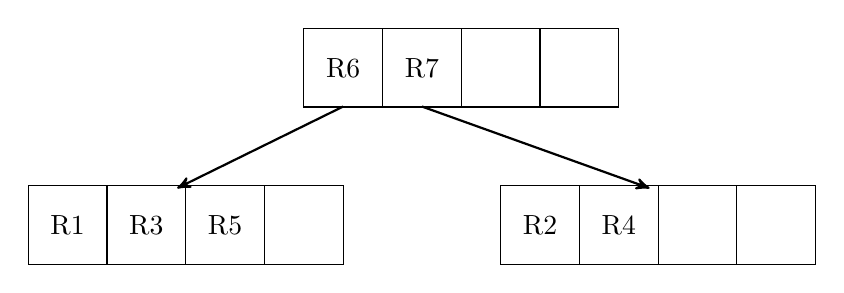
\begin{tikzpicture}
				\draw (-1.5,0) rectangle (-0.5,1) node[name=R6,pos=.5] {R6};
				\draw (-0.5,0) rectangle (0.5,1) node[name=R7,pos=.5] {R7};
				\draw (0.5,0) rectangle (1.5,1) node[name=D1,pos=.5] {};
				\draw (1.5,0) rectangle (2.5,1) node[name=D2,pos=.5] {};

				\draw (-5,-2) rectangle (-4,-1) node[name=R1,pos=.5] {R1};
				\draw (-4,-2) rectangle (-3,-1) node[name=R3,pos=.5] {R3};
				\draw (-3,-2) rectangle (-2,-1) node[name=R5,pos=.5] {R5};
				\draw (-2,-2) rectangle (-1,-1) node[name=D3,pos=.5] {};

				\draw (1,-2) rectangle (2,-1) node[name=R2,pos=.5] {R2};
				\draw (2,-2) rectangle (3,-1) node[name=R4,pos=.5] {R4};
				\draw (3,-2) rectangle (4,-1) node[name=D4,pos=.5] {};
				\draw (4,-2) rectangle (5,-1) node[name=D5,pos=.5] {};

				\node[fit=(R1)(R3)(R5)(D3)](leftLeaf){};
				\node[fit=(R2)(R4)(D4)(D5)](rightLeaf){};

				\draw [thick, ->, >=stealth']
				([yshift=-2.5mm]R6.south) -- ([yshift=1mm]leftLeaf.north);
				\draw [thick, ->, >=stealth']
				([yshift=-2.5mm]R7.south) -- ([yshift=1mm]rightLeaf.north);
			\end{tikzpicture}
		\end{center}


		\paragraph{Wie wählt man diese neuen Rechtecke am sinnvollsten aus?}

		Ziel sollte sein, die Wahrscheinlichkeit zu minimieren, dass bei einem lesenden Zugriff beide Rechtecke und damit beide Teilbäume durchsucht werden müssen.

		Dies erreicht man z.\,B. dadurch, dass die Gesamtfläche beider Rechtecke minimal gewählt wird.
		Dazu schlägt Guttman verschiedene Strategien vor, die hier nicht weiter diskutiert werden sollen.

		\paragraph{Einfügen von F}

		Um F einzufügen, muss geklärt werden, welcher Blattknoten gewählt wird.
		Wird F bzw. sein minimales umgebendes Rechteck in einen Blattknoten eingefügt, so müssen alle umgebenden Rechtecke auf dem Weg von der Wurzel bis zum neuen Eintrag vergrößert werden.
		Dabei ist die Grundidee beim Absteigen des Baumes immer denjenigen Weg zu wählen, auf dem das jeweilige umgebende Rechteck am wenigsten vergrößert werden muss.

		Der Knoten F sollte also in den linken Blattknoten eingefügt werden, da das Rechteck R6 nur leicht vergrößert werden muss.
		Würde man ihn in den rechten Blattknoten einfügen, müsste das Rechteck R7 vergrößert werden, das dann mehr als vier mal größer wäre als ursprünglich.

		\begin{center}
			\begin{tikzpicture}
				% border
				\draw (0,0) rectangle (6,6);

				\nodeA
				\nodeB
				\nodeC
				\nodeD
				\nodeE
				\nodeF

				\RA
				\RB
				\RC
				\RD
				\RE
				\RF


				% root node
				\draw[color=green] (0.4  , 1.2) rectangle (2.5, 5  ) node[anchor=south] {R6};
				\draw[color=green] (4.5, 2.0) rectangle (5.5, 4.8) node[anchor=south] {R7};

			\end{tikzpicture}
		\end{center}


		\begin{center}
			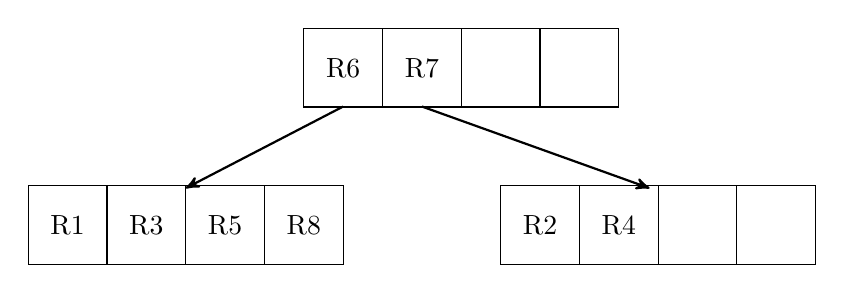
\begin{tikzpicture}
				\draw (-1.5,0) rectangle (-0.5,1) node[name=R6,pos=.5] {R6};
				\draw (-0.5,0) rectangle (0.5,1) node[name=R7,pos=.5] {R7};
				\draw (0.5,0) rectangle (1.5,1) node[name=D1,pos=.5] {};
				\draw (1.5,0) rectangle (2.5,1) node[name=D2,pos=.5] {};

				\draw (-5,-2) rectangle (-4,-1) node[name=R1,pos=.5] {R1};
				\draw (-4,-2) rectangle (-3,-1) node[name=R3,pos=.5] {R3};
				\draw (-3,-2) rectangle (-2,-1) node[name=R5,pos=.5] {R5};
				\draw (-2,-2) rectangle (-1,-1) node[name=D3,pos=.5] {R8};

				\draw (1,-2) rectangle (2,-1) node[name=R2,pos=.5] {R2};
				\draw (2,-2) rectangle (3,-1) node[name=R4,pos=.5] {R4};
				\draw (3,-2) rectangle (4,-1) node[name=D4,pos=.5] {};
				\draw (4,-2) rectangle (5,-1) node[name=D5,pos=.5] {};

				\node[fit=(R1)(R3)(R5)(D3)](leftLeaf){};
				\node[fit=(R2)(R4)(D4)(D5)](rightLeaf){};

				\draw [thick, ->, >=stealth']
				([yshift=-2.5mm]R6.south) -- ([yshift=1mm]leftLeaf.north);
				\draw [thick, ->, >=stealth']
				([yshift=-2.5mm]R7.south) -- ([yshift=1mm]rightLeaf.north);
			\end{tikzpicture}
		\end{center}

		\paragraph{Einfügen von G}

		Soll G eingefügt werden, entsteht ein Überlauf im linken Blattknoten, der zum Splitt führt.
		Dazu wird R6 verkleinert und ein neues Rechteck R10 aufgespannt.
		Die in R6 ursprünglich enthaltenen Einträge werden so verteilt, dass R6 und R10 jeweils mindestens $m$ Einträge enthalten und die Gesamtfläche von R6 und R10 möglichst klein ist.

		\begin{center}
			\begin{tikzpicture}
				% border
				\draw (0,0) rectangle (6,6);

				\nodeA
				\nodeB
				\nodeC
				\nodeD
				\nodeE
				\nodeF
				\nodeG

				\RA
				\RB
				\RC
				\RD
				\RE
				\RF
				\RG

				% root node
				\draw[color=green] (0.4, 2.7) rectangle (2.5, 5  ) node[anchor=south] {R6};
				\draw[color=green] (1.32, 0.5) rectangle (3.2, 2.2) node[anchor=south] {R10};
				\draw[color=green] (4.5, 2.0) rectangle (5.5, 4.8) node[anchor=south] {R7};

			\end{tikzpicture}
		\end{center}

		Der entstehende Baum sieht dann so aus:

		\begin{center}
			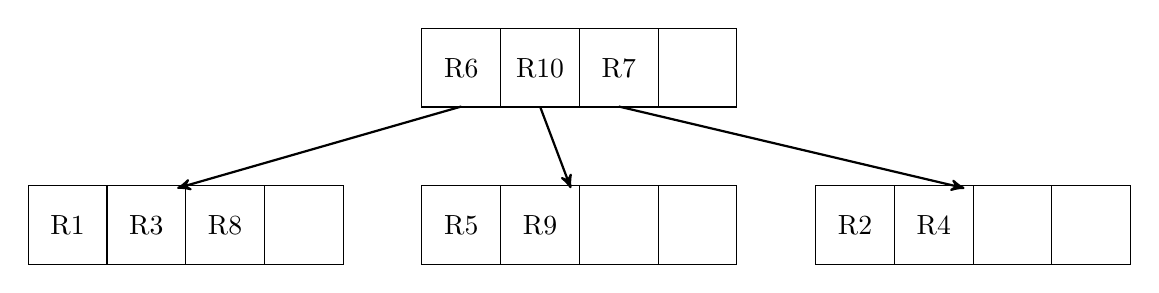
\begin{tikzpicture}
				\draw (0,0) rectangle (1,1) node[name=R6,pos=.5] {R6};
				\draw (1,0) rectangle (2,1) node[name=R10,pos=.5] {R10};
				\draw (2,0) rectangle (3,1) node[name=R7,pos=.5] {R7};
				\draw (3,0) rectangle (4,1) node[name=D2,pos=.5] {};

				\draw (-5,-2) rectangle (-4,-1) node[name=R1,pos=.5] {R1};
				\draw (-4,-2) rectangle (-3,-1) node[name=R3,pos=.5] {R3};
				\draw (-3,-2) rectangle (-2,-1) node[name=R8,pos=.5] {R8};
				\draw (-2,-2) rectangle (-1,-1) node[name=D3,pos=.5] {};

				\draw (0,-2) rectangle (1,-1) node[name=R5,pos=.5] {R5};
				\draw (1,-2) rectangle (2,-1) node[name=R9,pos=.5] {R9};
				\draw (2,-2) rectangle (3,-1) node[name=D4,pos=.5] {};
				\draw (3,-2) rectangle (4,-1) node[name=D5,pos=.5] {};

				\draw (5,-2) rectangle (6,-1) node[name=D6,pos=.5] {R2};
				\draw (6,-2) rectangle (7,-1) node[name=D7,pos=.5] {R4};
				\draw (7,-2) rectangle (8,-1) node[name=D8,pos=.5] {};
				\draw (8,-2) rectangle (9,-1) node[name=D9,pos=.5] {};

				\node[fit=(R1)(R3)(R8)(D3)](leftLeaf){};
				\node[fit=(R5)(R9)(D4)(D5)](centerLeaf){};
				\node[fit=(D6)(D7)(D8)(D9)](rightLeaf){};

				\draw [thick, ->, >=stealth']
				([yshift=-2.5mm]R6.south) -- ([yshift=1mm]leftLeaf.north);
				\draw [thick, ->, >=stealth']
				([yshift=-2.5mm]R10.south) -- ([yshift=1mm]centerLeaf.north);
				\draw [thick, ->, >=stealth']
				([yshift=-2.5mm]R7.south) -- ([yshift=1mm]rightLeaf.north);
			\end{tikzpicture}
		\end{center}

	\end{solution}
	\item Löschen Sie anschließend den Eintrag D.

	\begin{solution}
		Dies erzeugt einen Unterlauf im rechten Blattknoten.
		Nach Guttmans Algorithmus wird nun der gesamte Blattknoten und der Verweis auf ihn im Elternknoten gelöscht.
		Dadurch entsteht ein verwaister Eintrag (B in R2), dieser wird mit dem bereits bekannten Einfügealgorithmus erneut eingefügt.

		Dies ergibt folgendes Bild:

		\begin{center}
			\begin{tikzpicture}
				% border
				\draw (0,0) rectangle (6,6);

				\nodeA
				\nodeB
				\nodeC
				\nodeE
				\nodeF
				\nodeG

				\RA
				\RB
				\RC
				\RE
				\RF
				\RG

				% root node
				\draw[color=green] (0.4, 2.7) rectangle (5.5, 5  ) node[anchor=south] {R6};
				\draw[color=green] (1.32, 0.5) rectangle (3.2, 2.2) node[anchor=south] {R10};

			\end{tikzpicture}
		\end{center}


		\begin{center}
			\begin{tikzpicture}
				\draw (0,0) rectangle (1,1) node[name=R6,pos=.5] {R6};
				\draw (1,0) rectangle (2,1) node[name=R10,pos=.5] {R10};
				\draw (2,0) rectangle (3,1) node[name=R7,pos=.5] {};
				\draw (3,0) rectangle (4,1) node[name=D2,pos=.5] {};

				\draw (-5,-2) rectangle (-4,-1) node[name=R1,pos=.5] {R1};
				\draw (-4,-2) rectangle (-3,-1) node[name=R3,pos=.5] {R3};
				\draw (-3,-2) rectangle (-2,-1) node[name=R8,pos=.5] {R8};
				\draw (-2,-2) rectangle (-1,-1) node[name=D3,pos=.5] {R2};

				\draw (1,-2) rectangle (2,-1) node[name=R5,pos=.5] {R5};
				\draw (2,-2) rectangle (3,-1) node[name=R9,pos=.5] {R9};
				\draw (3,-2) rectangle (4,-1) node[name=D4,pos=.5] {};
				\draw (4,-2) rectangle (5,-1) node[name=D5,pos=.5] {};

				\node[fit=(R1)(R3)(R8)(D3)](leftLeaf){};
				\node[fit=(R5)(R9)(D4)(D5)](centerLeaf){};
				\node[fit=(D6)(D7)(D8)(D9)](rightLeaf){};

				\draw [thick, ->, >=stealth']
				([yshift=-2.5mm]R6.south) -- ([yshift=1mm]leftLeaf.north);
				\draw [thick, ->, >=stealth']
				([yshift=-2.5mm]R10.south) -- ([yshift=1mm]centerLeaf.north);
			\end{tikzpicture}
		\end{center}



	\end{solution}


\end{enumerate}


\beamertxt{\pagebreak}
\begin{deeper}
\section{R-Baum 2}
%% Vorlagen für die Zeichnungen
% circle radius
\newdimen\R
\R=0.5cm

\newcommand{\nodeAA} {
	\draw (4.5, 4.5) circle (\R) node {A};
}
\newcommand{\nodeBB} {
	\draw[xshift=1.0cm,yshift=3.3cm] (0:\R) \foreach \x in {72,144,...,359} {
		-- (\x:\R)
	} -- cycle (0:\R) node {B \hspace{0.8cm} } ;
}
\newcommand{\nodeCC} {
	\draw[xshift=0.8cm,yshift=1.7cm] (0:\R) \foreach \x in {120,240} {
		-- (\x:\R)
	} -- cycle (0:\R) node {C \hspace{0.9cm} } ;
}
\newcommand{\nodeDD} {
	\draw (0.7  , 4.5) circle (\R) node {D};
}
\newcommand{\nodeEE} {
	\draw (5.0, 1.0) circle (\R) node {E};
}
\newcommand{\nodeFF} {
	\draw[xshift=5.2cm,yshift=2.1cm] (0:\R) \foreach \x in {120,240} {
		-- (\x:\R)
	} -- cycle (0:\R) node {F \hspace{0.9cm} } ;
}
\newcommand{\nodeGG} {
	\draw (5.1, 3.3) circle (\R) node {G};
}
\newcommand{\nodeHH} {
	\draw (1.8, 5.3) circle (\R) node {H};
}
\newcommand{\nodeII} {
	\draw (1.9, 0.7) circle (\R) node {I};
}
\newcommand{\nodeJJ} {
	%\draw (2.4, 3.8) circle (\R) node {J};
	\draw[xshift=2.4cm,yshift=3.8cm] (0:\R) \foreach \x in {120,240} {
		-- (\x:\R)
	} -- cycle (0:\R) node {J \hspace{0.9cm} } ;
}


\newcommand{\RAA} {
	\draw (4  , 4  ) rectangle (5  , 5  ) node[pos=0.9,anchor=south east] {R1};
}
\newcommand{\RBB} {
	\draw (0.56, 2.8) rectangle (1.5, 3.8) node[pos=0.1,anchor=south east] {R2};
}
\newcommand{\RCC} {
	\draw (0.52, 2.2) rectangle (1.3, 1.2) node[pos=0.9,anchor=north east] {R3};
}
\newcommand{\RDD} {
	\draw (0.2, 4.0) rectangle (1.2, 5.0) node[pos=0.1,anchor=south east] {R4};
}
\newcommand{\REE} {
	\draw (4.5, 0.5) rectangle (5.5, 1.5) node[pos=0.1,anchor=north east] {R5};
}
\newcommand{\RFF} {
	\draw (4.92, 2.6) rectangle (5.7, 1.6) node[pos=0.2,anchor=north east] {R8};
}
\newcommand{\RGG} {
	\draw (4.6, 2.8) rectangle (5.6, 3.8) node[pos=0.2,anchor=north east] {R9};
}
\newcommand{\RHH} {
	\draw (1.3, 4.8) rectangle (2.3, 5.8) node[pos=0.9,anchor=north west] {R10};
}
\newcommand{\RII} {
	\draw (1.4, 0.2) rectangle (2.4, 1.2) node[pos=0.9,anchor=north west] {R11};
}
\newcommand{\RJJ} {
	\draw (2.12, 4.3) rectangle (2.9, 3.3) node[pos=0.9,anchor=north west] {R12};
}


Gegeben sei ein anfangs leerer R-Baum mit $M=4$ sowie die geometrischen Objekte A bis J im zweidimensionalen Raum.
Des Weiteren s wieder $m = \lfloor\frac{M}{2}\rfloor$:

\begin{center}
	\begin{tikzpicture}
		% border
		\draw (0,0) rectangle (6,6);

		\nodeAA
		\nodeBB
		\nodeCC
		\nodeDD
		\nodeEE
		\nodeFF
		\nodeGG
		\nodeHH
		\nodeII
		\nodeJJ

		%\RAA
		%\RBB
		%\RCC
		%\RDD
		%\REE
		%\RFF
		%\RGG
		%\RHH
		%\RII
		%\RJJ

	\end{tikzpicture}
\end{center}

\begin{enumerate}[a)]
	\item Fügen Sie die Einträge A bis E ein.

	\begin{note}
		Zunächst wird nur der Wurzelknoten gefüllt:
		\begin{center}
			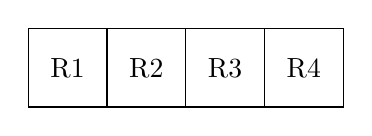
\begin{tikzpicture}
				\draw (0,0) rectangle (1,1) node[pos=.5] {R1};
				\draw (1,0) rectangle (2,1) node[pos=.5] {R2};
				\draw (2,0) rectangle (3,1) node[pos=.5] {R3};
				\draw (3,0) rectangle (4,1) node[pos=.5] {R4};
			\end{tikzpicture}
		\end{center}

		Die minimalen Rechtecke:
		\begin{center}
			\begin{tikzpicture}
				% border
				\draw (0,0) rectangle (6,6);

				\nodeAA
				\nodeBB
				\nodeCC
				\nodeDD

				\RAA
				\RBB
				\RCC
				\RDD
			\end{tikzpicture}
		\end{center}

		Durch E erfolgt der erste Splitt:


		Die minimalen Rechtecke:
		\begin{center}
			\begin{tikzpicture}
				% border
				\draw (0,0) rectangle (6,6);

				\nodeAA
				\nodeBB
				\nodeCC
				\nodeDD
				\nodeEE

				\RAA
				\RBB
				\RCC
				\RDD
				\REE

				% root node
				\draw[color=green] (0.2  , 1.2) rectangle (1.55, 5  ) node[anchor=south] {R6};
				\draw[color=green] (4.0, 0.5) rectangle (5.5, 5.0) node[anchor=south] {R7};
			\end{tikzpicture}
		\end{center}

		\begin{center}
			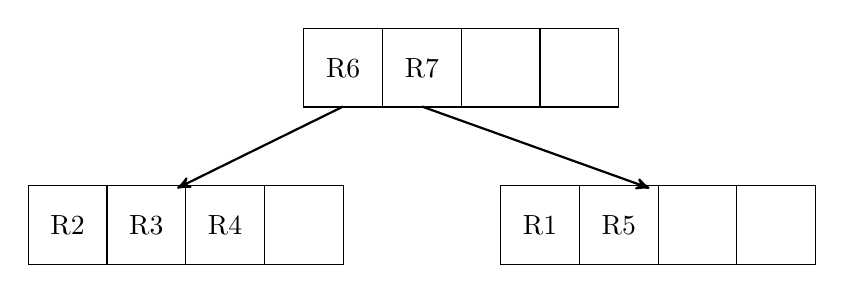
\begin{tikzpicture}
				\draw (-1.5,0) rectangle (-0.5,1) node[name=R6,pos=.5] {R6};
				\draw (-0.5,0) rectangle (0.5,1) node[name=R7,pos=.5] {R7};
				\draw (0.5,0) rectangle (1.5,1) node[name=D1,pos=.5] {};
				\draw (1.5,0) rectangle (2.5,1) node[name=D2,pos=.5] {};

				\draw (-5,-2) rectangle (-4,-1) node[name=R1,pos=.5] {R2};
				\draw (-4,-2) rectangle (-3,-1) node[name=R3,pos=.5] {R3};
				\draw (-3,-2) rectangle (-2,-1) node[name=R5,pos=.5] {R4};
				\draw (-2,-2) rectangle (-1,-1) node[name=D3,pos=.5] {};

				\draw (1,-2) rectangle (2,-1) node[name=R2,pos=.5] {R1};
				\draw (2,-2) rectangle (3,-1) node[name=R4,pos=.5] {R5};
				\draw (3,-2) rectangle (4,-1) node[name=D4,pos=.5] {};
				\draw (4,-2) rectangle (5,-1) node[name=D5,pos=.5] {};

				\node[fit=(R1)(R3)(R5)(D3)](leftLeaf){};
				\node[fit=(R2)(R4)(D4)(D5)](rightLeaf){};

				\draw [thick, ->, >=stealth']
				([yshift=-2.5mm]R6.south) -- ([yshift=1mm]leftLeaf.north);
				\draw [thick, ->, >=stealth']
				([yshift=-2.5mm]R7.south) -- ([yshift=1mm]rightLeaf.north);
			\end{tikzpicture}
		\end{center}

	\end{note}

	\item
	Löschen sie anschließend den Eintrag B.

	\begin{note}
		Der Knoten B, bzw. das minimale umgebende Rechteck R2, werden aus dem linken Blattknoten entfernt. Bei diesem Löschvorgang entsteht kein Unterlauf.
		\begin{center}
			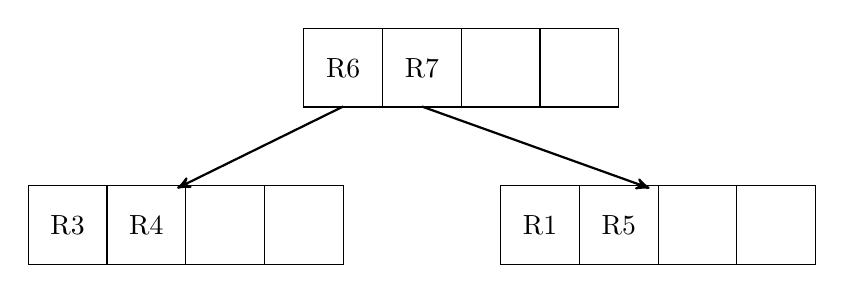
\begin{tikzpicture}
				\draw (-1.5,0) rectangle (-0.5,1) node[name=R6,pos=.5] {R6};
				\draw (-0.5,0) rectangle (0.5,1) node[name=R7,pos=.5] {R7};
				\draw (0.5,0) rectangle (1.5,1) node[name=D1,pos=.5] {};
				\draw (1.5,0) rectangle (2.5,1) node[name=D2,pos=.5] {};

				\draw (-5,-2) rectangle (-4,-1) node[name=R1,pos=.5] {R3};
				\draw (-4,-2) rectangle (-3,-1) node[name=R3,pos=.5] {R4};
				\draw (-3,-2) rectangle (-2,-1) node[name=R5,pos=.5] {};
				\draw (-2,-2) rectangle (-1,-1) node[name=D3,pos=.5] {};

				\draw (1,-2) rectangle (2,-1) node[name=R2,pos=.5] {R1};
				\draw (2,-2) rectangle (3,-1) node[name=R4,pos=.5] {R5};
				\draw (3,-2) rectangle (4,-1) node[name=D4,pos=.5] {};
				\draw (4,-2) rectangle (5,-1) node[name=D5,pos=.5] {};

				\node[fit=(R1)(R3)(R5)(D3)](leftLeaf){};
				\node[fit=(R2)(R4)(D4)(D5)](rightLeaf){};

				\draw [thick, ->, >=stealth']
				([yshift=-2.5mm]R6.south) -- ([yshift=1mm]leftLeaf.north);
				\draw [thick, ->, >=stealth']
				([yshift=-2.5mm]R7.south) -- ([yshift=1mm]rightLeaf.north);
			\end{tikzpicture}
		\end{center}

		Die minimalen Rechtecke:
		\begin{center}
			\begin{tikzpicture}
				% border
				\draw (0,0) rectangle (6,6);

				\nodeAA
				\nodeCC
				\nodeDD
				\nodeEE

				\RAA
				\RCC
				\RDD
				\REE

				% root node
				\draw[color=green] (0.2  , 1.2) rectangle (1.35, 5) node[anchor=south] {R6};
				\draw[color=green] (4.0, 0.5) rectangle (5.5, 5.0) node[anchor=south] {R7};
			\end{tikzpicture}
		\end{center}
	\end{note}

	\item
	Fügen sie anschließend die Einträge F bis J ein.

	\begin{note}
		Einfügen von Eintrag F:
		\begin{center}
			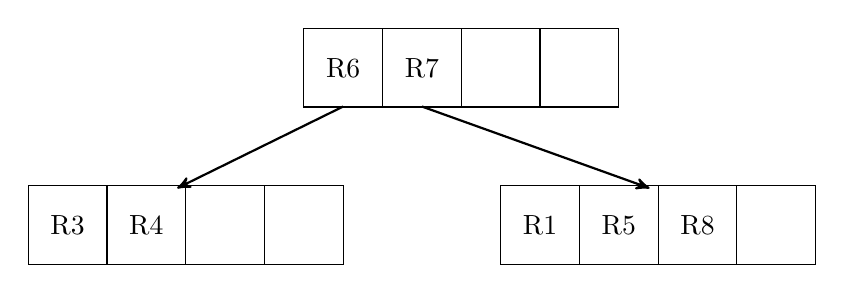
\begin{tikzpicture}
				\draw (-1.5,0) rectangle (-0.5,1) node[name=R6,pos=.5] {R6};
				\draw (-0.5,0) rectangle (0.5,1) node[name=R7,pos=.5] {R7};
				\draw (0.5,0) rectangle (1.5,1) node[name=D1,pos=.5] {};
				\draw (1.5,0) rectangle (2.5,1) node[name=D2,pos=.5] {};

				\draw (-5,-2) rectangle (-4,-1) node[name=R1,pos=.5] {R3};
				\draw (-4,-2) rectangle (-3,-1) node[name=R3,pos=.5] {R4};
				\draw (-3,-2) rectangle (-2,-1) node[name=R5,pos=.5] {};
				\draw (-2,-2) rectangle (-1,-1) node[name=D3,pos=.5] {};

				\draw (1,-2) rectangle (2,-1) node[name=R2,pos=.5] {R1};
				\draw (2,-2) rectangle (3,-1) node[name=R4,pos=.5] {R5};
				\draw (3,-2) rectangle (4,-1) node[name=D4,pos=.5] {R8};
				\draw (4,-2) rectangle (5,-1) node[name=D5,pos=.5] {};

				\node[fit=(R1)(R3)(R5)(D3)](leftLeaf){};
				\node[fit=(R2)(R4)(D4)(D5)](rightLeaf){};

				\draw [thick, ->, >=stealth']
				([yshift=-2.5mm]R6.south) -- ([yshift=1mm]leftLeaf.north);
				\draw [thick, ->, >=stealth']
				([yshift=-2.5mm]R7.south) -- ([yshift=1mm]rightLeaf.north);
			\end{tikzpicture}
		\end{center}

		Die minimalen Rechtecke:
		\begin{center}
			\begin{tikzpicture}
				% border
				\draw (0,0) rectangle (6,6);

				\nodeAA
				\nodeCC
				\nodeDD
				\nodeEE
				\nodeFF

				\RAA
				\RCC
				\RDD
				\REE
				\RFF

				% root node
				\draw[color=green] (0.2  , 1.2) rectangle (1.35, 5) node[anchor=south] {R6};
				\draw[color=green] (4.0, 0.5) rectangle (5.7, 5.0) node[anchor=south] {R7};
			\end{tikzpicture}
		\end{center}

		Einfügen von Eintrag G:
		\begin{center}
			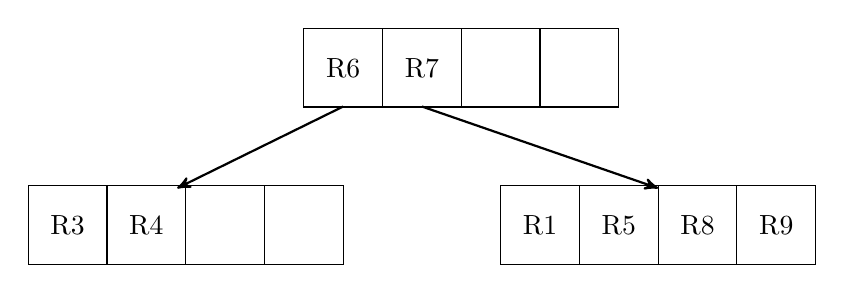
\begin{tikzpicture}
				\draw (-1.5,0) rectangle (-0.5,1) node[name=R6,pos=.5] {R6};
				\draw (-0.5,0) rectangle (0.5,1) node[name=R7,pos=.5] {R7};
				\draw (0.5,0) rectangle (1.5,1) node[name=D1,pos=.5] {};
				\draw (1.5,0) rectangle (2.5,1) node[name=D2,pos=.5] {};

				\draw (-5,-2) rectangle (-4,-1) node[name=R1,pos=.5] {R3};
				\draw (-4,-2) rectangle (-3,-1) node[name=R3,pos=.5] {R4};
				\draw (-3,-2) rectangle (-2,-1) node[name=R5,pos=.5] {};
				\draw (-2,-2) rectangle (-1,-1) node[name=D3,pos=.5] {};

				\draw (1,-2) rectangle (2,-1) node[name=R2,pos=.5] {R1};
				\draw (2,-2) rectangle (3,-1) node[name=R4,pos=.5] {R5};
				\draw (3,-2) rectangle (4,-1) node[name=D4,pos=.5] {R8};
				\draw (4,-2) rectangle (5,-1) node[name=D5,pos=.5] {R9};

				\node[fit=(R1)(R3)(R5)(D3)](leftLeaf){};
				\node[fit=(R2)(R4)(D4)(D5)](rightLeaf){};

				\draw [thick, ->, >=stealth']
				([yshift=-2.5mm]R6.south) -- ([yshift=1mm]leftLeaf.north);
				\draw [thick, ->, >=stealth']
				([yshift=-2.5mm]R7.south) -- ([yshift=1mm]rightLeaf.north);
			\end{tikzpicture}
		\end{center}

		Die minimalen Rechtecke:
		\begin{center}
			\begin{tikzpicture}
				% border
				\draw (0,0) rectangle (6,6);

				\nodeAA
				\nodeCC
				\nodeDD
				\nodeEE
				\nodeFF
				\nodeGG

				\RAA
				\RCC
				\RDD
				\REE
				\RFF
				\RGG

				% root node
				\draw[color=green] (0.2  , 1.2) rectangle (1.35, 5) node[anchor=south] {R6};
				\draw[color=green] (4.0, 0.5) rectangle (5.7, 5.0) node[anchor=south] {R7};
			\end{tikzpicture}
		\end{center}

		Einfügen von Eintrag H:
		\begin{center}
			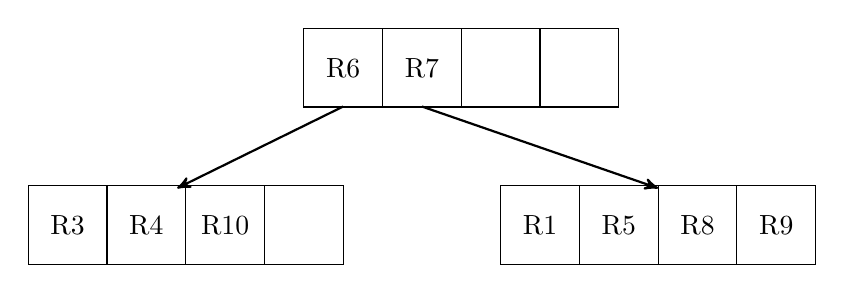
\begin{tikzpicture}
				\draw (-1.5,0) rectangle (-0.5,1) node[name=R6,pos=.5] {R6};
				\draw (-0.5,0) rectangle (0.5,1) node[name=R7,pos=.5] {R7};
				\draw (0.5,0) rectangle (1.5,1) node[name=D1,pos=.5] {};
				\draw (1.5,0) rectangle (2.5,1) node[name=D2,pos=.5] {};

				\draw (-5,-2) rectangle (-4,-1) node[name=R1,pos=.5] {R3};
				\draw (-4,-2) rectangle (-3,-1) node[name=R3,pos=.5] {R4};
				\draw (-3,-2) rectangle (-2,-1) node[name=R5,pos=.5] {R10};
				\draw (-2,-2) rectangle (-1,-1) node[name=D3,pos=.5] {};

				\draw (1,-2) rectangle (2,-1) node[name=R2,pos=.5] {R1};
				\draw (2,-2) rectangle (3,-1) node[name=R4,pos=.5] {R5};
				\draw (3,-2) rectangle (4,-1) node[name=D4,pos=.5] {R8};
				\draw (4,-2) rectangle (5,-1) node[name=D5,pos=.5] {R9};

				\node[fit=(R1)(R3)(R5)(D3)](leftLeaf){};
				\node[fit=(R2)(R4)(D4)(D5)](rightLeaf){};

				\draw [thick, ->, >=stealth']
				([yshift=-2.5mm]R6.south) -- ([yshift=1mm]leftLeaf.north);
				\draw [thick, ->, >=stealth']
				([yshift=-2.5mm]R7.south) -- ([yshift=1mm]rightLeaf.north);
			\end{tikzpicture}
		\end{center}

		Die minimalen Rechtecke:
		\begin{center}
			\begin{tikzpicture}
				% border
				\draw (0,0) rectangle (6,6);

				\nodeAA
				\nodeCC
				\nodeDD
				\nodeEE
				\nodeFF
				\nodeGG
				\nodeHH

				\RAA
				\RCC
				\RDD
				\REE
				\RFF
				\RGG
				\RHH

				% root node
				\draw[color=green] (0.2  , 1.2) rectangle (2.35, 5.8) node[anchor=south] {R6};
				\draw[color=green] (4.0, 0.5) rectangle (5.7, 5.0) node[anchor=south] {R7};
			\end{tikzpicture}
		\end{center}

		Einfügen von Eintrag I:
		\begin{center}
			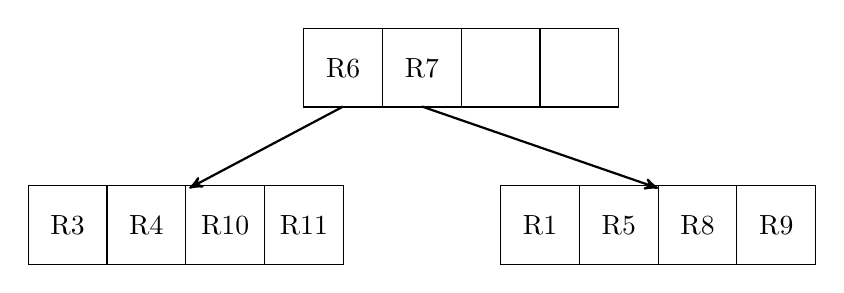
\begin{tikzpicture}
				\draw (-1.5,0) rectangle (-0.5,1) node[name=R6,pos=.5] {R6};
				\draw (-0.5,0) rectangle (0.5,1) node[name=R7,pos=.5] {R7};
				\draw (0.5,0) rectangle (1.5,1) node[name=D1,pos=.5] {};
				\draw (1.5,0) rectangle (2.5,1) node[name=D2,pos=.5] {};

				\draw (-5,-2) rectangle (-4,-1) node[name=R1,pos=.5] {R3};
				\draw (-4,-2) rectangle (-3,-1) node[name=R3,pos=.5] {R4};
				\draw (-3,-2) rectangle (-2,-1) node[name=R5,pos=.5] {R10};
				\draw (-2,-2) rectangle (-1,-1) node[name=D3,pos=.5] {R11};

				\draw (1,-2) rectangle (2,-1) node[name=R2,pos=.5] {R1};
				\draw (2,-2) rectangle (3,-1) node[name=R4,pos=.5] {R5};
				\draw (3,-2) rectangle (4,-1) node[name=D4,pos=.5] {R8};
				\draw (4,-2) rectangle (5,-1) node[name=D5,pos=.5] {R9};

				\node[fit=(R1)(R3)(R5)(D3)](leftLeaf){};
				\node[fit=(R2)(R4)(D4)(D5)](rightLeaf){};

				\draw [thick, ->, >=stealth']
				([yshift=-2.5mm]R6.south) -- ([yshift=1mm]leftLeaf.north);
				\draw [thick, ->, >=stealth']
				([yshift=-2.5mm]R7.south) -- ([yshift=1mm]rightLeaf.north);
			\end{tikzpicture}
		\end{center}

		Die minimalen Rechtecke:
		\begin{center}
			\begin{tikzpicture}
				% border
				\draw (0,0) rectangle (6,6);

				\nodeAA
				\nodeCC
				\nodeDD
				\nodeEE
				\nodeFF
				\nodeGG
				\nodeHH
				\nodeII

				\RAA
				\RCC
				\RDD
				\REE
				\RFF
				\RGG
				\RHH
				\RII

				% root node
				\draw[color=green] (0.2  , 0.2) rectangle (2.4, 5.8) node[anchor=south] {R6};
				\draw[color=green] (4.0, 0.5) rectangle (5.7, 5.0) node[anchor=south] {R7};

			\end{tikzpicture}
		\end{center}

		Einfügen von Eintrag J:
		\begin{center}
			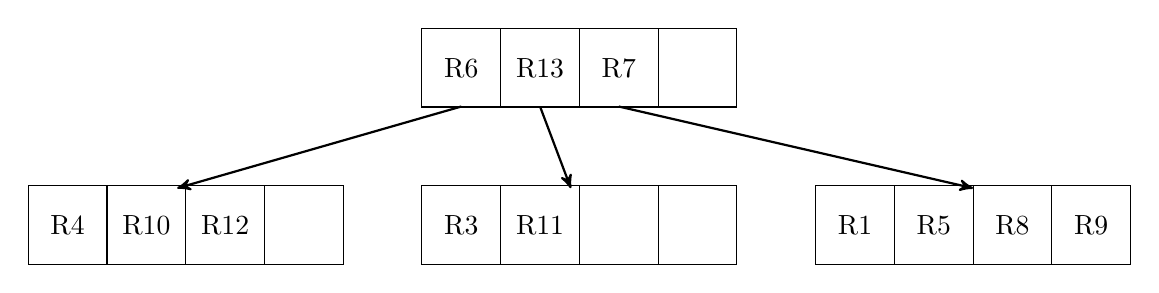
\begin{tikzpicture}
				\draw (0,0) rectangle (1,1) node[name=R6,pos=.5] {R6};
				\draw (1,0) rectangle (2,1) node[name=R10,pos=.5] {R13};
				\draw (2,0) rectangle (3,1) node[name=R7,pos=.5] {R7};
				\draw (3,0) rectangle (4,1) node[name=D2,pos=.5] {};

				\draw (-5,-2) rectangle (-4,-1) node[name=R1,pos=.5] {R4};
				\draw (-4,-2) rectangle (-3,-1) node[name=R3,pos=.5] {R10};
				\draw (-3,-2) rectangle (-2,-1) node[name=R8,pos=.5] {R12};
				\draw (-2,-2) rectangle (-1,-1) node[name=D3,pos=.5] {};

				\draw (0,-2) rectangle (1,-1) node[name=R5,pos=.5] {R3};
				\draw (1,-2) rectangle (2,-1) node[name=R9,pos=.5] {R11};
				\draw (2,-2) rectangle (3,-1) node[name=D4,pos=.5] {};
				\draw (3,-2) rectangle (4,-1) node[name=D5,pos=.5] {};

				\draw (5,-2) rectangle (6,-1) node[name=D6,pos=.5] {R1};
				\draw (6,-2) rectangle (7,-1) node[name=D7,pos=.5] {R5};
				\draw (7,-2) rectangle (8,-1) node[name=D8,pos=.5] {R8};
				\draw (8,-2) rectangle (9,-1) node[name=D9,pos=.5] {R9};

				\node[fit=(R1)(R3)(R8)(D3)](leftLeaf){};
				\node[fit=(R5)(R9)(D4)(D5)](centerLeaf){};
				\node[fit=(D6)(D7)(D8)(D9)](rightLeaf){};

				\draw [thick, ->, >=stealth']
				([yshift=-2.5mm]R6.south) -- ([yshift=1mm]leftLeaf.north);
				\draw [thick, ->, >=stealth']
				([yshift=-2.5mm]R10.south) -- ([yshift=1mm]centerLeaf.north);
				\draw [thick, ->, >=stealth']
				([yshift=-2.5mm]R7.south) -- ([yshift=1mm]rightLeaf.north);
			\end{tikzpicture}
		\end{center}

		Die minimalen Rechtecke:
		\begin{center}
			\begin{tikzpicture}
				% border
				\draw (0,0) rectangle (6,6);

				\nodeAA
				\nodeCC
				\nodeDD
				\nodeEE
				\nodeFF
				\nodeGG
				\nodeHH
				\nodeII
				\nodeJJ

				\RAA
				\RCC
				\RDD
				\REE
				\RFF
				\RGG
				\RHH
				\RII
				\RJJ

				% root node
				\draw[color=green] (0.2, 3.3) rectangle (2.9, 5.8) node[anchor=south] {R6};
				\draw[color=green] (4.0, 0.5) rectangle (5.7, 5.0) node[anchor=south] {R7};
				\draw[color=green] (0.5, 0.2) rectangle (2.4, 2.2) node[anchor=south] {R13};
			\end{tikzpicture}
		\end{center}
	\end{note}

	\item
	Löschen sie anschließend die Einträge D und I.

	\begin{note}
		Löschen von Eintrag D:
		\begin{center}
			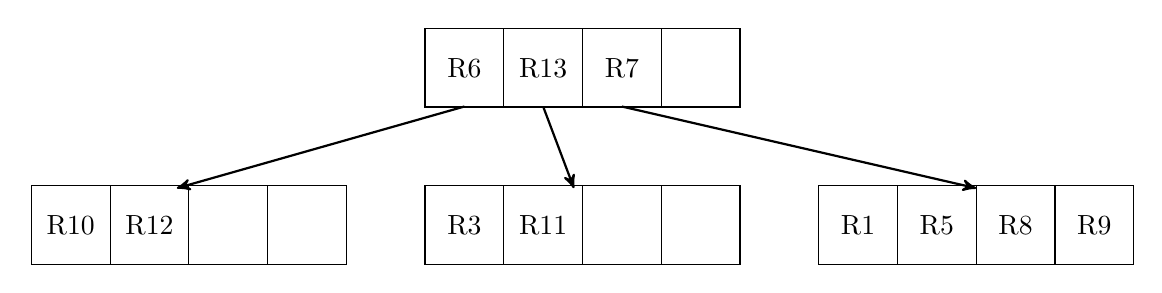
\begin{tikzpicture}
				\draw (0,0) rectangle (1,1) node[name=R6,pos=.5] {R6};
				\draw (1,0) rectangle (2,1) node[name=R10,pos=.5] {R13};
				\draw (2,0) rectangle (3,1) node[name=R7,pos=.5] {R7};
				\draw (3,0) rectangle (4,1) node[name=D2,pos=.5] {};

				\draw (-5,-2) rectangle (-4,-1) node[name=R1,pos=.5] {R10};
				\draw (-4,-2) rectangle (-3,-1) node[name=R3,pos=.5] {R12};
				\draw (-3,-2) rectangle (-2,-1) node[name=R8,pos=.5] {};
				\draw (-2,-2) rectangle (-1,-1) node[name=D3,pos=.5] {};

				\draw (0,-2) rectangle (1,-1) node[name=R5,pos=.5] {R3};
				\draw (1,-2) rectangle (2,-1) node[name=R9,pos=.5] {R11};
				\draw (2,-2) rectangle (3,-1) node[name=D4,pos=.5] {};
				\draw (3,-2) rectangle (4,-1) node[name=D5,pos=.5] {};

				\draw (5,-2) rectangle (6,-1) node[name=D6,pos=.5] {R1};
				\draw (6,-2) rectangle (7,-1) node[name=D7,pos=.5] {R5};
				\draw (7,-2) rectangle (8,-1) node[name=D8,pos=.5] {R8};
				\draw (8,-2) rectangle (9,-1) node[name=D9,pos=.5] {R9};

				\node[fit=(R1)(R3)(R8)(D3)](leftLeaf){};
				\node[fit=(R5)(R9)(D4)(D5)](centerLeaf){};
				\node[fit=(D6)(D7)(D8)(D9)](rightLeaf){};

				\draw [thick, ->, >=stealth']
				([yshift=-2.5mm]R6.south) -- ([yshift=1mm]leftLeaf.north);
				\draw [thick, ->, >=stealth']
				([yshift=-2.5mm]R10.south) -- ([yshift=1mm]centerLeaf.north);
				\draw [thick, ->, >=stealth']
				([yshift=-2.5mm]R7.south) -- ([yshift=1mm]rightLeaf.north);
			\end{tikzpicture}
		\end{center}

		Die minimalen Rechtecke:
		\begin{center}
			\begin{tikzpicture}
				% border
				\draw (0,0) rectangle (6,6);

				\nodeAA
				\nodeCC
				\nodeEE
				\nodeFF
				\nodeGG
				\nodeHH
				\nodeII
				\nodeJJ

				\RAA
				\RCC
				\REE
				\RFF
				\RGG
				\RHH
				\RII
				\RJJ

				% root node
				\draw[color=green] (1.3, 3.3) rectangle (2.9, 5.8) node[anchor=south] {R6};
				\draw[color=green] (4.0, 0.5) rectangle (5.7, 5.0) node[anchor=south] {R7};
				\draw[color=green] (0.5, 0.2) rectangle (2.4, 2.2) node[anchor=south] {R13};
			\end{tikzpicture}
		\end{center}

		Löschen von Eintrag I:
		\begin{center}
			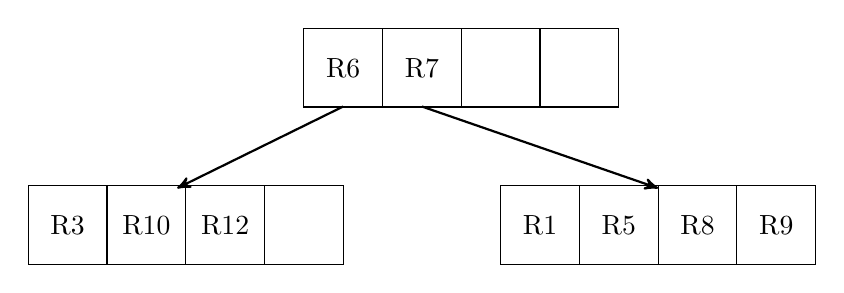
\begin{tikzpicture}
				\draw (-1.5,0) rectangle (-0.5,1) node[name=R6,pos=.5] {R6};
				\draw (-0.5,0) rectangle (0.5,1) node[name=R7,pos=.5] {R7};
				\draw (0.5,0) rectangle (1.5,1) node[name=D1,pos=.5] {};
				\draw (1.5,0) rectangle (2.5,1) node[name=D2,pos=.5] {};

				\draw (-5,-2) rectangle (-4,-1) node[name=R1,pos=.5] {R3};
				\draw (-4,-2) rectangle (-3,-1) node[name=R3,pos=.5] {R10};
				\draw (-3,-2) rectangle (-2,-1) node[name=R5,pos=.5] {R12};
				\draw (-2,-2) rectangle (-1,-1) node[name=D3,pos=.5] {};

				\draw (1,-2) rectangle (2,-1) node[name=R2,pos=.5] {R1};
				\draw (2,-2) rectangle (3,-1) node[name=R4,pos=.5] {R5};
				\draw (3,-2) rectangle (4,-1) node[name=D4,pos=.5] {R8};
				\draw (4,-2) rectangle (5,-1) node[name=D5,pos=.5] {R9};

				\node[fit=(R1)(R3)(R5)(D3)](leftLeaf){};
				\node[fit=(R2)(R4)(D4)(D5)](rightLeaf){};

				\draw [thick, ->, >=stealth']
				([yshift=-2.5mm]R6.south) -- ([yshift=1mm]leftLeaf.north);
				\draw [thick, ->, >=stealth']
				([yshift=-2.5mm]R7.south) -- ([yshift=1mm]rightLeaf.north);
			\end{tikzpicture}
		\end{center}

		Die minimalen Rechtecke:
		\begin{center}
			\begin{tikzpicture}
				% border
				\draw (0,0) rectangle (6,6);

				\nodeAA
				\nodeCC
				\nodeEE
				\nodeFF
				\nodeGG
				\nodeHH
				\nodeJJ

				\RAA
				\RCC
				\REE
				\RFF
				\RGG
				\RHH
				\RJJ

				% root node
				\draw[color=green] (0.5, 1.2) rectangle (2.9, 5.8) node[anchor=south] {R6};
				\draw[color=green] (4.0, 0.5) rectangle (5.7, 5.0) node[anchor=south] {R7};
			\end{tikzpicture}
		\end{center}
	\end{note}

\end{enumerate}

\end{deeper}

\beamertxt{\pagebreak}
\section{Function Based Index}
\begin{enumerate}[a)]
\item \label{item:fbi} Betrachten Sie folgenden Ausschnitt aus der Relation \textit{sortiment}:

\begin{center}
$\begin{tabular}{cc|c|c|c}
~&\underline{artikelnummer} & bezeichnung & nettopreis & mwst\_satz\\
\cline{2-5} \\
\textit{1}: & 110242 & Rechenblock & 0,99 & 0,07\\
\textit{2}: & 000815 & Datenbanken leicht gemacht & 24,89 & 0,07\\
\textit{3}: & 546813 & 15 Inner-Joins & 10,00 & 0,19\\
\textit{4}: & 123123 & Datenbankfestplatte & 149,99 & 0,19\\
~ & ... & ... & ... & ...
\end{tabular}$
\end{center}

Wie können Anfragen, die Produkte mit einem bestimmten Bruttopreis ermitteln, beschleunigt werden?

\begin{note}
Nicht aus der Vorlesung bekannt.
\end{note}

\begin{solution}
Eine Möglichkeit sind die zusätzliche Speicherung des Bruttopreises und das Anlegen eines Indexes über diesem Attribut.
Dies hat allerdings den gravierenden Nachteil der Redundanz.
Wenn das Attribut nicht automatisch berechnet wird, können widersprüchliche Daten abgelegt werden.
Außerdem wird das Schema zum Zwecke der Optimierung verändert und diese somit nach außen sichtbar.
Bestehende Anfragen müssten geändert werden, damit sie von dem neuen Index profitieren.

Eine Lösung, die diese Probleme nicht hat, ist ein Index, der als Schlüssel einen berechneten Wert verwendet, der nicht in der Datenbank gespeichert ist.
Einen solchen Index nennt man Function Based Index.
Als Indexstruktur kann z.\,B. ein B-Baum oder ein Hashindex verwendet werden.

Im vorliegenden Fall wird ein Function Based Index über den Bruttopreis benötigt.

\paragraph{Zusatzfrage} Wie lauten die Funktion für den Function Based Index und wie die Schlüssel zu jedem Tupel der Beispieltabelle, die im Index abgelegt werden?

Funktion:
\begin{equation*}
bruttopreis~ =~ nettopreis~ \cdot~ (1 + mwst\_satz)
\end{equation*}

Zu Zeile \textit{1}: 1,06

Zu Zeile \textit{2}: 26,63

Zu Zeile \textit{3}: 11,90

Zu Zeile \textit{4}: 178,49
\end{solution}

\item Bei welcher Art von Anfragen und bei welchem Nutzungsverhalten ist der Einsatz eines Function Based Index sinnvoll?

\begin{solution}
Der Einsatz eines solchen Index ist sinnvoll, wenn nach bestimmten Werten, wie dem Bruttopreis im Beispiel, die sich zwar aus anderen Attributen berechnen lassen, allerdings nicht in der Relation gespeichert sind, häufig gefiltert oder sortiert wird.

Ein Function Based Index beschleunigt nur Abfragen, die den Wert des Function Based Index benötigen.
Wie jeder Index muss dieser beim Einfügen und Ändern angepasst und dabei die Funktion erneut berechnet werden.
Dies verlangsamt die Einfüge- und Änderungsoperationen. Es muss also auch bei diesem Indextyp abgewogen werden, ob der Nutzen des Index den Pflegeaufwand rechtfertigt.

Bei Einfügen und Ändern kann die Aktualisierung des Function Based Index abhängig von der Funktion übermäßig viel Zeit beanspruchen, da z.\,B. die Analyse von Bildern, Videos oder Audiodateien sehr aufwändig sein kann.
\end{solution}

\item Diskutieren Sie weitere Beispiele, die ähnliche Anforderungen haben wie das aus Teilaufgabe \ref{item:fbi}). Denken Sie dabei etwa an Multimedia-Anwendungen.

\begin{solution}
Ein möglicher Einsatz ist ein Function Based Index über die durchschnittliche Helligkeit eines Bildes oder über die Frequenzverteilung eines Audiostücks.

Ein Beispiel für den praktischen Einsatz eines Function Based Index (in Oracle) findet sich unter folgendem Link:\\
\url{https://docs.oracle.com/cd/E11882\_01/server.112/e40540/indexiot.htm\#CNCPT1161}.

\end{solution}

\end{enumerate}


\beamertxt{\pagebreak}
\section{Einordnung}
\begin{itemize}
	\item Wie sieht das Schichtenmodell vom Beginn der Vorlesung inzwischen aus?
	\item Welche Strukturen werden in den jeweiligen Schichten verwendet?
	\item Wie wird jede Schicht von der darüber liegenden adressiert? Wie adressiert sie selbst?
\end{itemize}

\begin{solution}
Ein paar Stichworte zur Diskussion (am Ende sollte eine Grafik ähnlich der auf Folie~\SchichtVLFuenf~oder~\SchichtVLSechs~entstanden sein):
\begin{itemize}
	\item interne Satzschnittstelle
	\item blockorientierte Schnittstelle
	\item Satzverwaltung
	\item Externspeicherverwaltung
	\item Kanalkommandos
\end{itemize}

\includegraphics[width=14cm]{Pictures/Ue06_Aufgabe3_1.png}

Einfügen einer seitenorientierten Pufferschnittstelle, Details im nächsten Übungsblatt:

\includegraphics[width=14cm]{Pictures/Ue06_Aufgabe3_2.png}

\end{solution}


\beamertxt{\pagebreak}
\begin{deeper}
\section{Programmieraufgabe 4: HashImpl}

\subsection{Aufgabenstellung}
\begin{enumerate}
	\item Implementieren Sie eine Klasse, die die Schnittstelle \beamertxt{\linebreak}\texttt{idb.record.KeyRecordFile} implementiert.
		Beachten Sie die Dokumentation der Methoden in der Schnittstelle. Beachten Sie, dass diese Aufgabe den Übungsaufgaben zum Thema Lineares Hashing entspricht.
		Ihre Implementierung soll dieses Verhalten umsetzen.
	\item Tragen Sie den Konstruktor Ihrer Klasse in \texttt{idb.construct.Util} in der Methode \texttt{generateHash()} ein.
		Die Funktion soll den DBBuffer und zwei BlockFiles nehmen (eine zusätzliche für den Überlaufbereich) und eine \textbf{neue} HashImpl zurückgeben.
		Beachten Sie, dass die BlockFiles zu diesem Zeitpunkt schon geöffnet sind.
		Die zusätzlichen Parameter \texttt{threshhold, initCapacity} entsprechen den für das Lineare Hashing bekannten Parametern.
	\item Tragen Sie den Konstruktor Ihrer Klasse in \texttt{idb.construct.Util} in der Methode \texttt{rebuildHash()} ein.
		Die Funktion soll den DBBuffer und zwei BlockFiles nehmen und eine \textbf{existierende} HashImpl vom Laufwerk laden.
		Beachten Sie, dass die BlockFiles zu diesem Zeitpunkt schon geöffnet sind.
		Beachten Sie auch, dass Sie \texttt{threshhold, initCapacity} und eventuelle interne Zustände wieder vom Laufwerk rekonstruieren müssen.
		Anders als bei einer TID speichern wir diese hier ab, anstatt sie beim Laden neu zu berechnen.
	\item Sorgen Sie dafür, dass Sie alle Tests aus der Klasse \texttt{HashTests} erfüllen. Warnung: Diese Testfälle können 1-2 Minuten dauern.
	Sie können diese Testfälle mit \lstinline|ant Meilenstein4| ausführen.
	\item Die Abgabe auf GitLab erfolgt zeitgleich mit der Abgabe der Zusatzaufgaben des nächsten Übungsblattes auf StudOn. Markieren Sie hierfür ihre Abgabe mit dem Tag "`Aufgabe-4"'.
\end{enumerate}

\subsection{Hinweise}
\begin{itemize}
	\item Wir empfehlen, den ersten Block des Overflow-Bereiches für Metadaten zu verwenden und erst ab dem zweiten Block im Overflow-Bereich Hashing zu betreiben.
	\item \texttt{KeyRecordFile} bietet eine Methode \texttt{close()}, in der diese Metadaten serialisiert werden können.
		Es wird sichergestellt, dass nicht zwei verschiedene \mbox{HashImpl} auf den gleichen Dateien arbeiten.
	\item Im Rahmen dieser Aufgabe ist die Behandlung von Sätzen, die länger als ein (halber) Block sind, nicht notwenig. (Dies liegt daran, dass wir diese \texttt{HashImpl} nur als Sekundärindex nutzen werden.)
	\item Es empfiehlt sich, in jedem Block Platz für einen \texttt{int} freizuhalten, um dort ggf. einen Zeiger auf einen anderen Block einzutragen.
	\item Initial müssen üblicherweise neue Blöcke (in \texttt{append()} oder im Konstruktor) mindestens partiell initialisiert werden, damit nicht beliebige Daten als Zeiger o. Ä. interpretiert werden.
	\item Im Gegensatz zu TID kann man sich im \texttt{HashImpl} darauf verlassen, dass \texttt{Key.copy} jegliche Keys und \texttt{Value.copy} jegliche Values lesen und wieder serialisieren können.
	\item Achten Sie darauf, beim Einfügen und beim Split die Reihenfolgeeigenschaften in \texttt{idb.record.KeyRecordFile:insert} nicht zu verletzen.
	\item \textbf{Bonus:} Implementieren Sie eine einfache Freispeicherverwaltung für die Blöcke im Overflowbereich. Diese ist besonders einfach, da jeder Block genau gleich groß ist.
	\item Im Gegensatz zu Blöcken im Speicher können Daten die in ein \texttt{DataObject} geladen wurden problemlos nach Freigabe des Blockes verwendet werden.
	\item Achten Sie darauf, nicht zu viele Datensätze gleichzeitig aus den Blöcken in ein \texttt{DataObject} zu konvertieren. In einem echten System geht hierbei leicht der RAM aus.
	\item Folgende Hilfsmethode sind vermutlich ganz nützlich: \texttt{int hash(Key), int alloc(), void free(), List<Triplet<Key, DataObject, Integer>> listBlockContest(ByteBuffer)}
	\item Vermutlich ist es hilfreich, sich zu notieren, wie viel Platz in einem Block noch frei ist.
	\item Für \texttt{split()} ist es nötig, die Anzahl an insgesamt belegten Bytes zu kennen.
\end{itemize}

\end{deeper}

\end{document}

